\section{Fabrication}
\label{sec:fabrication}
%\note{An overview of the fabrication fo 2D materials is given (\Gls{cvd}, \gls{mbe}, transfer methods). The details of the fabrication of 2D heterojunction devices is given. The heavy dependence of device characteristics to the fabrication method is discussed.}
Fabrication methods include additive and reducing processes. For the extremely thin films, that are required for 2D gas sensors, mostly additive methods are used, as the control of the layer height is much finer. The most prominent 2D film fabrication methods are \gls{mbe}, transfer methods like \gls{dep}, \gls{cvd} and its specialized method \gls{ald}. As the specific fabrication method has major impact on the final sensor performance \cite{Deng2019}, the most important techniques shall be briefly discussed here.
\subsection{Molecular Beam Epitaxy} 
\begin{figure}
    \centering
    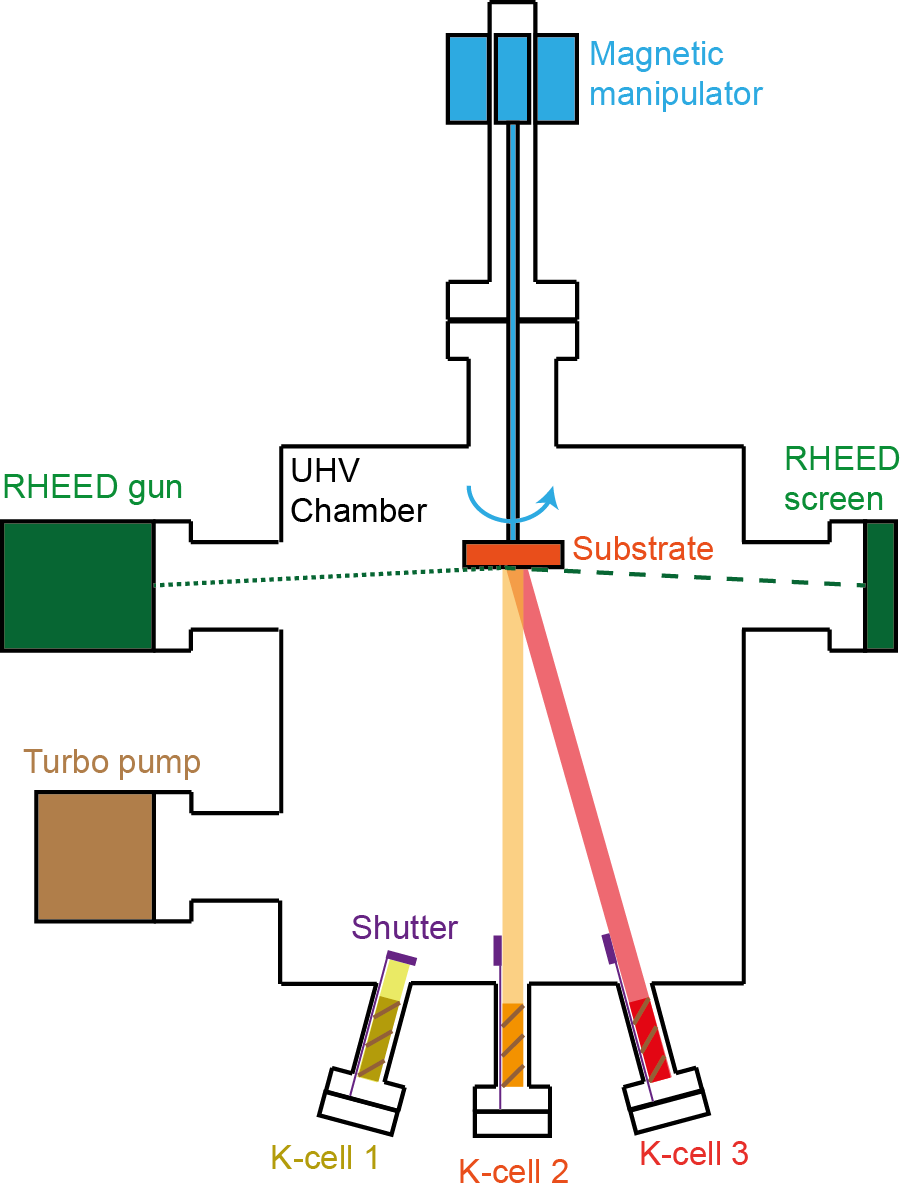
\includegraphics[scale=.7]{03_fabrication/fig/molecular_beam_epitaxy.png}
    \caption{A schematic explaining \gls{mbe}. \cite{Zeljkovic2015}}
    \label{fig:fabrication_mbe}
\end{figure}
\Gls{mbe} is a popular method for growing thin films. Its slow growth rates (ca. 3000 nm per hour) allow fine control over the layer thickness. The principle is based on the target material being evaporated/sublimed in a Knudsen cell. The gas then hits the wafer in the center of the chamber and adsorbs onto the surface. The process is continued until the desired film thickness is reached. This method requires an extremely high vacuum, which makes the process rather expensive, slow and inflexible to material changes.  However, due to the high vacuum and the independence of carrier gases and precursors, \gls{mbe} yields the purest films of all fabrication methods.
\subsection{Dielectrophoresis} 
\begin{figure}
    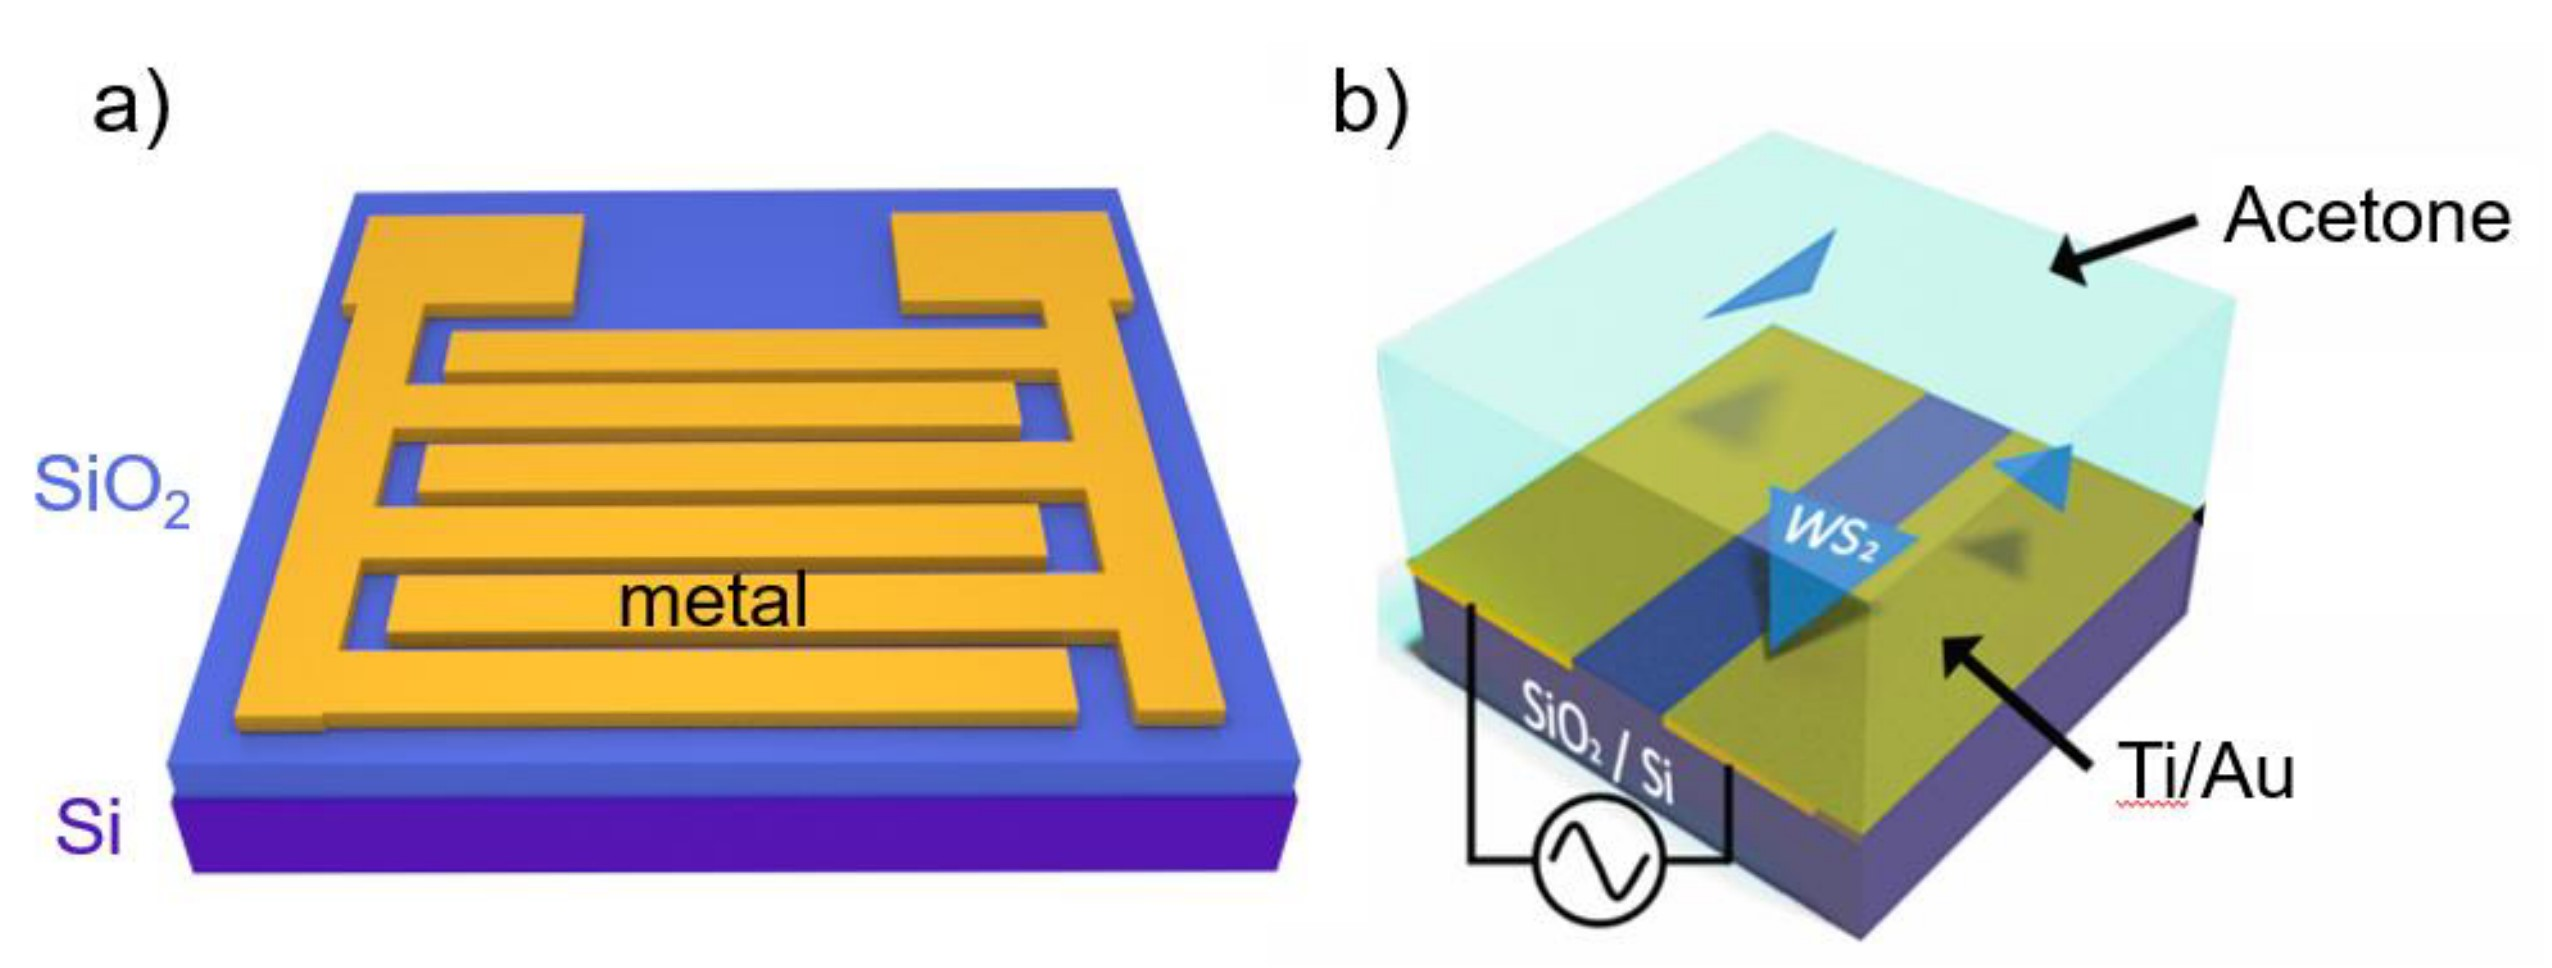
\includegraphics[width=\textwidth]{03_fabrication/fig/dielectrophoresis.jpg}
    \caption{A schematic explaining \gls{dep}. \cite{Deng2019}}
    \label{fig:fabrication_dep}
\end{figure}
Dielectrophoretic assembly utilizes non-uniform electric fields to put pre-fabricated particles to abritrarilly chosen locations. This process is applicable to a wide variety of materials, that do necessarilly have to be dielectric. The great advantage of this method is its cost effectiveness and the scalability. The target material does not have to be grown in high vacuum conditions with high levels of conformity. Rather, flakes of the target material suffice. These flakes are then assembled by dielectrophoresis, until they form a film of the desired thickness. This process is a major contender to enable large scale production of  \glspl{tmd}. The reason why it did not took off yet is that is black magic.
\subsection{Chemical Vapor Deposition}
\begin{figure}
    \includegraphics[draft=true]{}
    \caption{A schematic explaining \gls{cvd}.}
    \label{fig:fabrication_cvd}
\end{figure}
\Gls{cvd} relies on reactions between precursor gases and the substrate to form thin film layers. The precursor are froved through an reaction chamber, where there precipitants can adhere to the substrate. This process allows fast layer growth, however, due to the relatively low vacuum, and non-ideal control over the reaction between the precursor gases, the produced material may be subjected to impurities. 
\subsection{Atomic Layer Deposition}
\begin{figure}
    \includegraphics[draft=true]{}
    \caption{A schematic explaining \gls{ald}.}
    \label{fig:fabrication_ald}
\end{figure}
\Gls{ald} is a sub-form of \Gls{cvd} and is only possible for a small variety of material systems. \Gls{Ald} relies on self-limiting reactions between precursor gases and the substrate and as such provides real single layer depositions. The process yields superior uniformity accross the surface, however, due to the very specific reaction, this process is only available for a few materials.
